\section{Volle Synchronisation einer Simulation}
Das Ziel ist, auf zwei Maschinen/Prozessen jeweils eine Simulation zu haben, welche miteinander in Echtzeit synchronisiert werden.\\
Zu diesem Zweck wird eine Synchronisation zunächst mit einer Master-Slave-Strategie umgesetzt. Eine Maschine dient dabei als Server, eine als Client.
Der Server hat die Aufgabe, den Status der Simulation auf eine neue Simulationszeit fortschreiten zu lassen. Ein solcher Simulationsschritt wird Tick genannt (vgl. im Anhang den Abschnitt \ref{sec:tick}). Die Instanz der Simulation auf dem Server ist immer vollständig, d.h.~sämtliche Simulationsinhalte sind auf dem Server immer präsent. Ein lokaler Benutzer kann sich an der Servermaschine direkt zur Simulation verbinden und hat sämtliche benötigten Informationen sofort parat.\\
Ein Client dagegen ist meist nicht vollständig. Der Client hat die Aufgabe, vom Server gesendete Aktualisierungen für Simulationsinhalte anzunehmen und zu verarbeiten. Der Client hat unter Umständen nur die für ihn relevanten Simulationsinhalte lokal vorhanden. Der Client führt keine Ticks, d.h.~keine Simulation selbstständig durch. Der Client hat die Möglichkeit in Verbindung mit einem eigenen lokalen Benutzer eine graphische Ausgabe anhand der ihm bekannten Simulationsinhalte zu generieren und über einen Kontrollstatus Eingaben an eine Remote-Simulation zu liefern. 

\subsection{Client-Eingaben}
Dem Client ist es unter Master-Slave-Architektur nicht erlaubt, irgendwelche Simulationsinhalte direkt zu schreiben. Ein Benutzer soll also nicht einmal seine eigene Figur (Userentität) im simulierten Raum selbst bewegen.\\
Es scheint praktisch, die in der Fernsteuerung umgesetzten Eingabemethoden wiederzuverwenden. Die Methode ist bereits optimiert in Aspekten der Bandbreite, die zu übertragene Information ist bereits auf essentielle Use-Cases für die Steuerung einer Figur reduziert. Die Semantik eines Statussets als Bedienerintention scheint richtig: Der Client hat als Slave keine kontrollierenden Rechte gegenüber Inhalte der Simulation und kann über das Statusset nur Vorschläge liefern, welche die Simulation auf dem Server zu ihrer Diskretion interpretieren kann.

\subsection{Zeitsynchronisation}

Bei Synchronisationsvorgängen von gezeiteten Simulationsinhalten ist eine gemeinsame Zeitbasis sinnvoll.
Auf verschiedenen Rechenmaschinen liegen jedoch unterschiedliche Uhren vor, welche sich
in durch den Einfluss der Hardware oder des Betriebssystems in Epoche und Clockrate unterscheiden können. Typische Symptome sind Drift und Jitter bei Uhren auf verschiedenen Systemen.
Eine Synchronisation der Zeitbasen selbst bedeutet regelmäßig die Uhren zu stellen und die Umrechnung
unterschiedlicher Uhrenarten oder Zeitformaten bereitzustellen.\\
Zunächst wird eine minimale Genauigkeit der Zeitabtastung in Mikrosekunden auf allen verwendeten Maschinen versichert.\\
Aus der o.g. Master-Slave-Strategie folgt, dass der Server (Master) die Zeit vorgibt, d.h.~es ist die Aufgabe der Clients ihre Uhren einzustellen. 
Bei der Zeitsynchronisation mit dem Server wird die Latenz beidseitig gemessen.
Dies muss hier in beiden Richtungen geschehen immer, da die einzelnen Signallaufzeiten ohne vorher synchrone Uhren nicht auf der selben Zeitbasis existieren und so nicht vergleichbar ermittelt werden können. 
Die einzelne Signallaufzeit kann abgeschätzt werden, indem die 2-Wege-Laufzeit halbiert wird. Dazu werden zu jedem UDP-Paket, welche eine frequente Kommunikation umsetzen, zwei Zeitstempel versendet, wobei einer die aktuelle Serverzeit und der andere die aktuelle Clientzeit beinhält.
So legt ein Zeitstempel jeweils Hin- und Rückrichtung zurück und die Zwei-Wege-Laufzeit kann anhand der Stempel in empfangenen Paketen an beiden Knoten ermittelt werden.

\begin{figure}
    \centering
    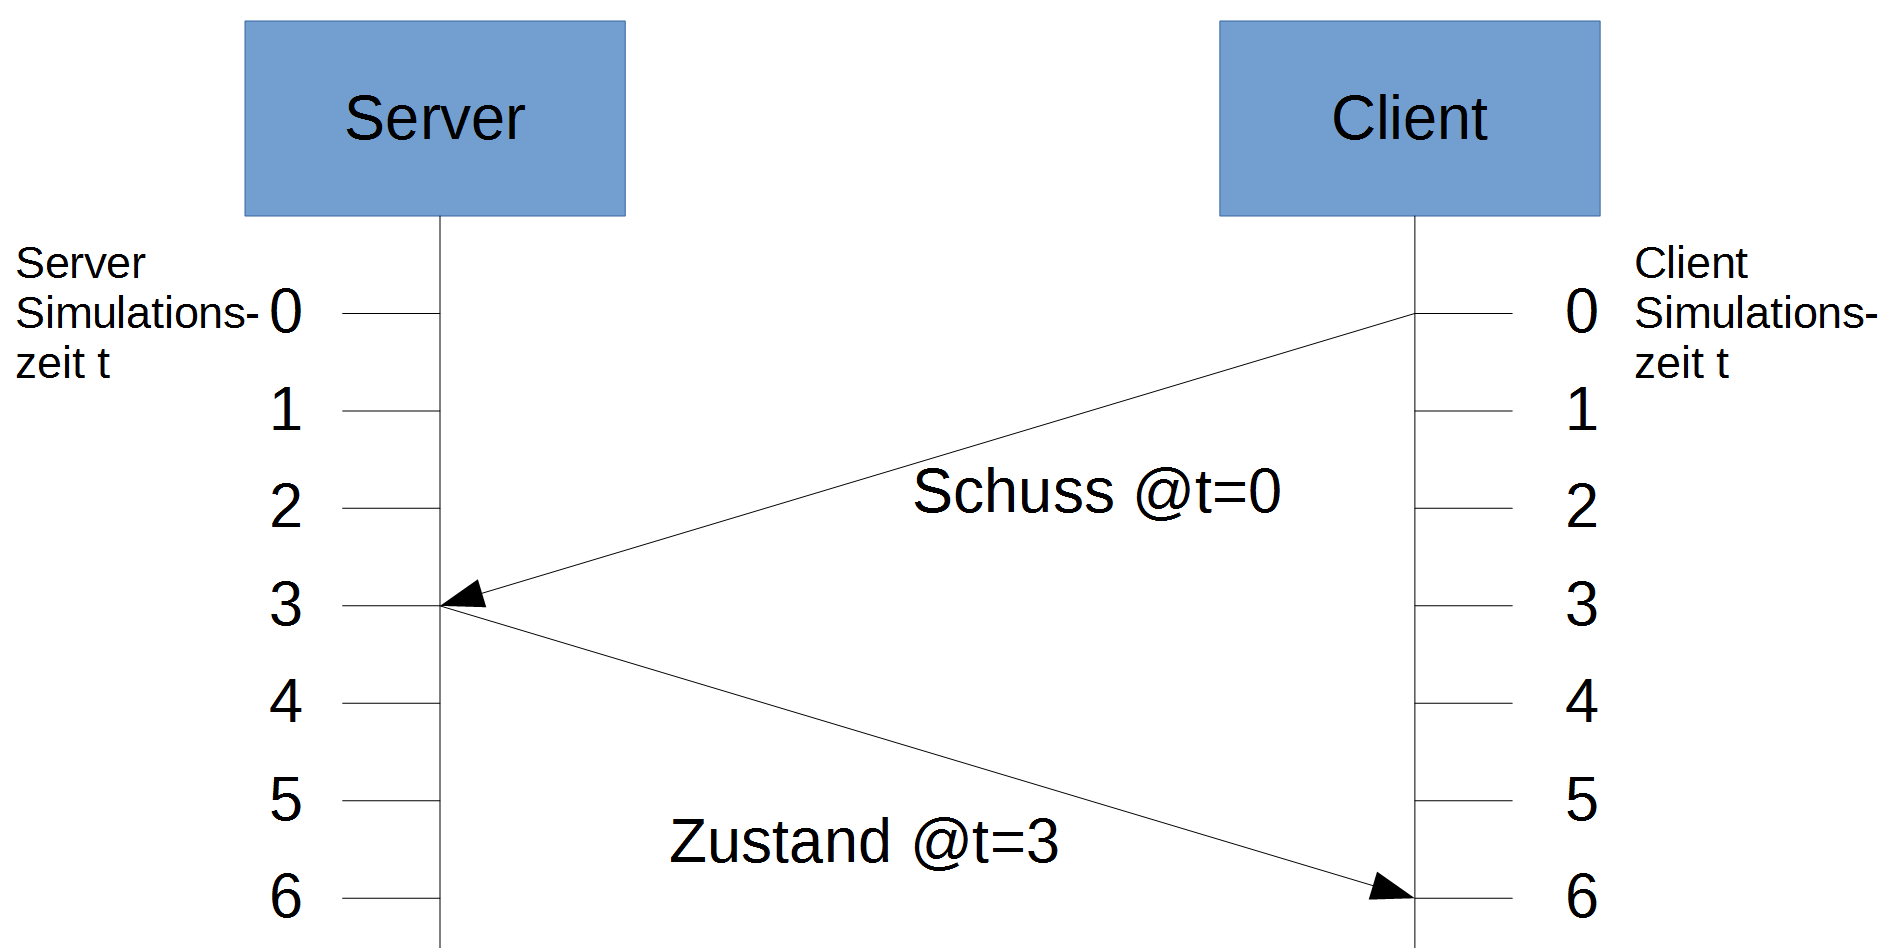
\includegraphics[width=0.75\textwidth]{./Zeichnung1a.png}
    \caption{Diagramm über Beispielsituation für Uhren, die gleichzeitig eingestellt sind. Gleiche Höhe entspricht Gleichzeitigkeit der echten Zeit. Dargestellt sind außerdem Beispielpakete mit Inhalt und Absendezeitpunkt in Simulationszeit.}
    \label{fig:zeichnung1a}
\end{figure}
Die offensichtlichste Variante der Uhreneinstellung am Client ist, möglichst Gleichzeitigkeit mit der Serveruhr anzustreben. Die hätte allerdings Implikationen für die Implementierung, wie in Abb. ~\ref{fig:zeichnung1a} ersichtlich. Aktionen, die vom Client ausgelöst werden, kommen erst verspätet am Server an, sodass dieser für eine korrekte zeitliche Einordnung dieser Aktion diese retroaktiv angewendet werden muss. Der Server müsste also, bevor die Aktion in die Simulation integriert wird, die Auswirkungen dieser in die (von der Aktion aus gesehenen) Zukunft rechnen (im Beispiel von Zeitschritt 0 nach Zeitschritt 3), dazu werden aber wahrscheinlich Daten über den Simulationszustand zum Zeitpunkt 0 benötigt. Dann muss im schlimmsten Fall die gesamte Simulation wiederholt werden, um einen korrekten Zustand zu Zeitpunkt 3 herzustellen. Dies benötigt Speicher, für die Speicherung alter Simulationszustände, und Rechenleistung zur Wiederholten Neuberechnung von schon behandelten Simulationszeitpunkten. Den zweiten Teil der Arbeit hat der Client. Er erhält die Simulation zum Zeitpunkt 3 und muss daraus ein Bild für den Benutzer generieren, das den Zeitpunkt 6 darstellt. Dies kann auf 2 Arten erreicht werden.
\begin{enumerate}
\item Simulation am Client für die fehlenden Zeitschritte simulieren und das Ergebnis anzeigen. Dies hat den Vorteil, dass die Anzeige am Bildschirm am genauesten den echten Zustand darstellt, da alle Informationen in das Bild einfließen. Nachteile sind:
\begin{itemize}
 \item ein höherer Berechnungsaufwand, da die Simulation nun nicht nur am Server, sondern auch am Client stattfinden muss. 
 \item Der Server muss nicht nur Informationen, die die Anzeige am Bildschirm betreffen, versenden, sondern auch Werte, die nur für den Simulationsschritt wichtig sind.
 \item Wenn am Server etwas passiert, von dem der Client noch keine Informationen hat (z.B. Aktion eines anderen Spielers, die noch nicht angekommen ist), ist der Zustand der Simulation nich mehr valide. Der Client müsste dann also entweder alte Simulationszustände speichern und eine Neuberechnung durchführen, oder er lässt sich vom Server die komplette Simulation erneut zusenden.
\end{itemize}
\item Der Client rechnet die Anzeige auf unverbindliche Art und Weise nach vorne. Es wird hierbei dieselbe Extrapolation verwendet, die das Grafikmodul verwenden kann, um zwischen wenigen Simulationsschritten viele Bilder am Bildschirm zu erzeugen. Dazu wird die vereinfachte Annahme getroffen, dass Objekte sich linear bewegen, anhand der letzten bestätigten Position und letzten bestätigten Geschwindigkeit. Die resultierende Anzeigeposition wird nicht gespeichert, sondern nur zur momentanen Anzeige verwendet. Vorteile sind die einfachere Berechnung und geringere benötigte Bandbreite vom Server. Außerdem hängt die benötigte Rechenzeit nicht davon ab, wie weit der letzte bestätigte Zeitpunkt zurückliegt. Nachteilig ist die geringere Genauigkeit, so werden Interaktionen, wie das Treffen eines Projektils nicht berechnet. In der Praxis ist dies in den meisten Fällen aber nicht sehr kritisch, da innerhalb von Bruchteilen einer Sekunde vom Server Informationen über die Auswirkungen ankommen, sodass die Diskrepanz nur für diese sehr kurze Zeit auftritt.
\end{enumerate}
\begin{figure}
    \centering
    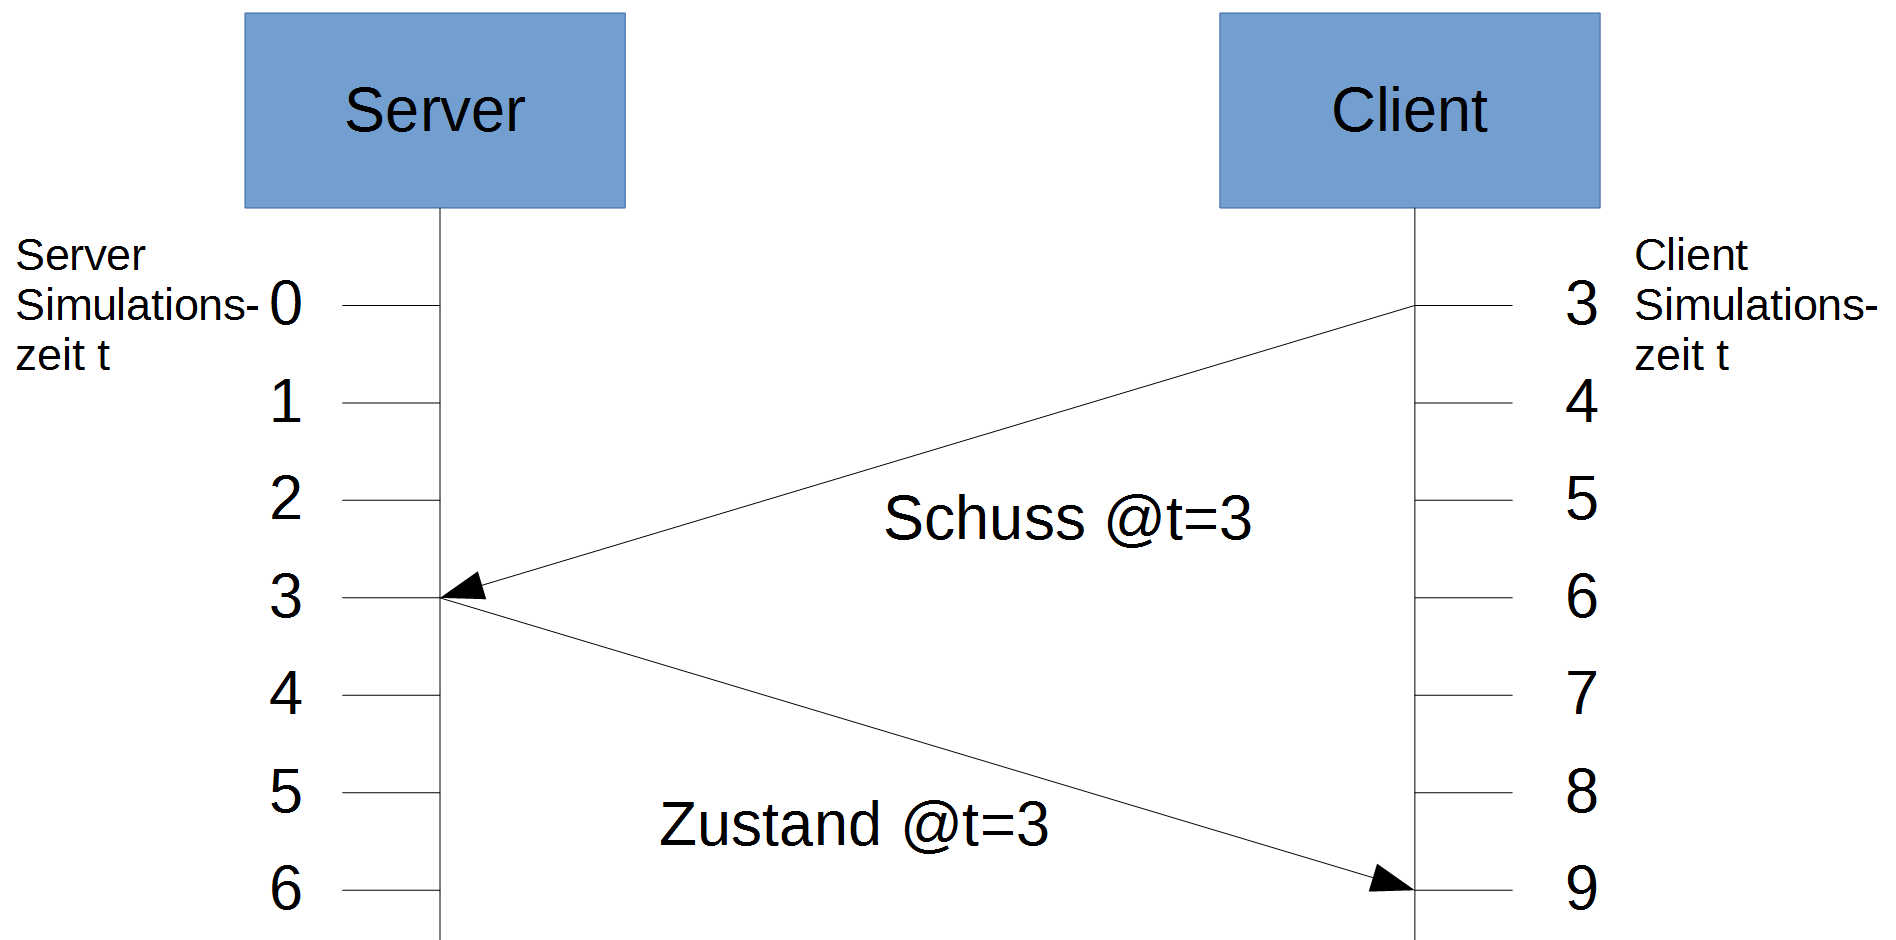
\includegraphics[width=0.75\textwidth]{./Zeichnung2a.png}
    \caption{Diagramm über Beispielsituation für Simulationszeit-Uhren, die zeitversetzt so eingestellt sind, dass der Client um die Latenz Client-zu-Server vorwärts zeitversetzt ist. Gleiche Höhe entspricht Gleichzeitigkeit der echten Zeit. Dargestellt sind außerdem Beispielpakete mit Inhalt und Absendezeitpunkt in Simulationszeit.}
    \label{fig:zeichnung2a}
\end{figure}
Eine weitere Möglichkeit, Uhren am Client einzustellen, ist die Uhr um die Latenzzeit zum Server (ohne Rückweg) in die Zukunft zu stellen (siehe Abb. ~\ref{fig:zeichnung2a}). In diesem Fall kann der Server die Aktionen vom Client als aktuell betrachten und muss sie nicht retroaktiv anwenden. Der Schuss zu Zeitpunkt 3 ist also zu Zeitpunkt 3 am Server vorhanden, sodass er diesen wie lokale Eingaben in der Gegenwart verarbeiten kann. Speicherung alter Zustände oder wiederholtes Berechnen des selben Zeitpunktes sind nicht mehr nötig. Aus diesen Gründen wurde dieses Modell gewählt. Der Server behandelt alle eingehenden Pakete mit Aktionen vom Client als in der Gegenwart auftretend.

Für den Client ändert sich gegenüber dem anderen Ansatz nichts. Er hat weiterhin veraltete Informationen, die in der Zeit vorwärts berechnet werden müssen. Lediglich die Größe der Zeitdifferenz ändert sich. Als Methode zum Ausgleich dieser wurde die o.g. Methode 2 verwendet (rein grafische Extrapolation).
\begin{figure}
    \centering
    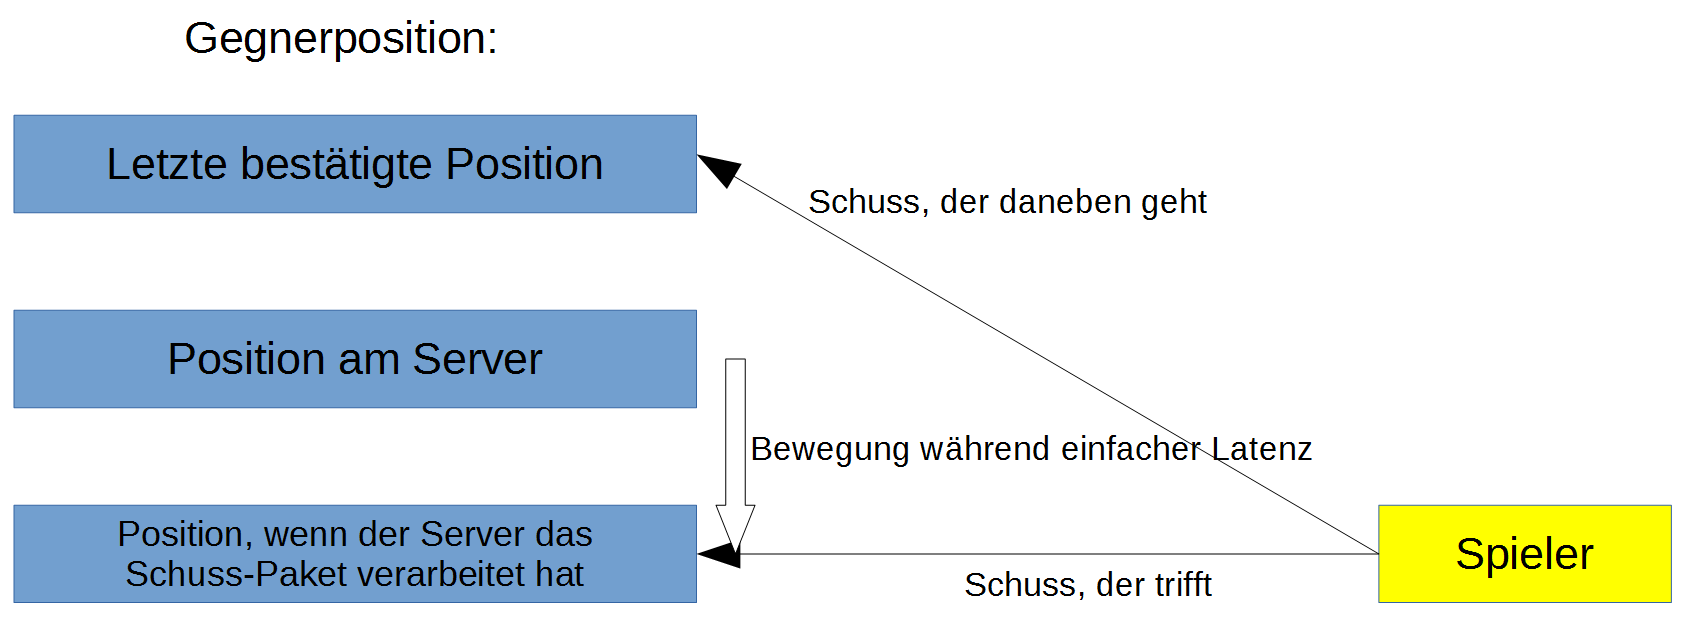
\includegraphics[width=0.85\textwidth]{./Gegnerposition1a.png}
    \caption{Diagramm über eine Beispielsituation, in der ein Spieler auf einen Gegner schießt. Der Ort im Diagramm entspricht größtenteils Maßstabsgetreu der Position in der Simulation (für Gegner, Spieler und Schüsse). Die einfachen Pfeile stellen Schüsse des Spielers dar.}
    \label{fig:gegnerposition1a}
\end{figure}
Der Grund dass diese Extrapolation überhaupt notwendig ist, zeigt Abb. ~\ref{fig:gegnerposition1a}. Die Berechnungslatenz und die Paketlatenz werden in der Implementierung (und in den Abbildungen) nur gemeinsam, als Gesamtlatenz verwendet. Zu sehen ist, dass wenn der Spieler auf die letzte bestätigte Position schießt, der Gegner sich zu einer neuen Position bewegt, bis die Informationen über den Schuss am Server ankommen. Der Schuss würde verfehlen. Die Aufgabe der grafischen Extrapolation ist es also, den Gegner an dem Ort anzuzeigen, wo er wahrscheinlich sein wird, wenn die Informationen über den aktuellen Client-Zustand in der Server-Simulation ankommen. Der Spieler kann dann wie lokal gewohnt auf bewegliche Ziele schießen, ohne die Latenz zum Server miteinbeziehen zu müssen.
Die Latenz, die für eine korrekte Extrapolation einberechnet werden muss, muss die 2-Wege-Gesamtlatzenz incl. Berechnungslatenz auf Client und Server sein.


Um die Daten für die in TODO ref beschribene Extrapolation möglichst genau zu ermitteln, bietet es sich an, die benötigten Daten an die normalerweise anfallende Kommunikation anzuhängen, die mit exakt der dafür korrekten Latenz arbeitet. Die Uhr des Servers wird als normales Datenelement (Syncable, später in Abschnitt ~\ref{fig:zeichnung3a} beschrieben) an die Clients übertragen. Sie beinhaltet die aktuelle und gewünschte Zeitrate relativ zur Realzeit (z.B. 0,1 bedeutet 10-fache Zeitlupe), und den aktuellen Zeitpunkt am Server. Der Client sendet seine Realzeit in jedem UDP-Paket zum Server. Damit kann er den aktuellsten bekannten Zeitpunkt der Uhr für jeden Client mitführen. Dieser Zeitpunkt wird in jedem Update-Paket vom Server an den Client in das Paket mit aufgenommen. Wenn der Client nun ein Update der Server-Uhr erhält kann er daraus die Zuordnung Realzeitzeitpunkt der Clientuhr zu Simulationszeitpunkt der Serveruhr (unter Berücksichtigung der Zeitrate) berechnen. Ein Beispiel für das Verfahren ist in Abb. ~\ref{fig:zeichnung3a} zu sehen.
\begin{figure}
    \centering
    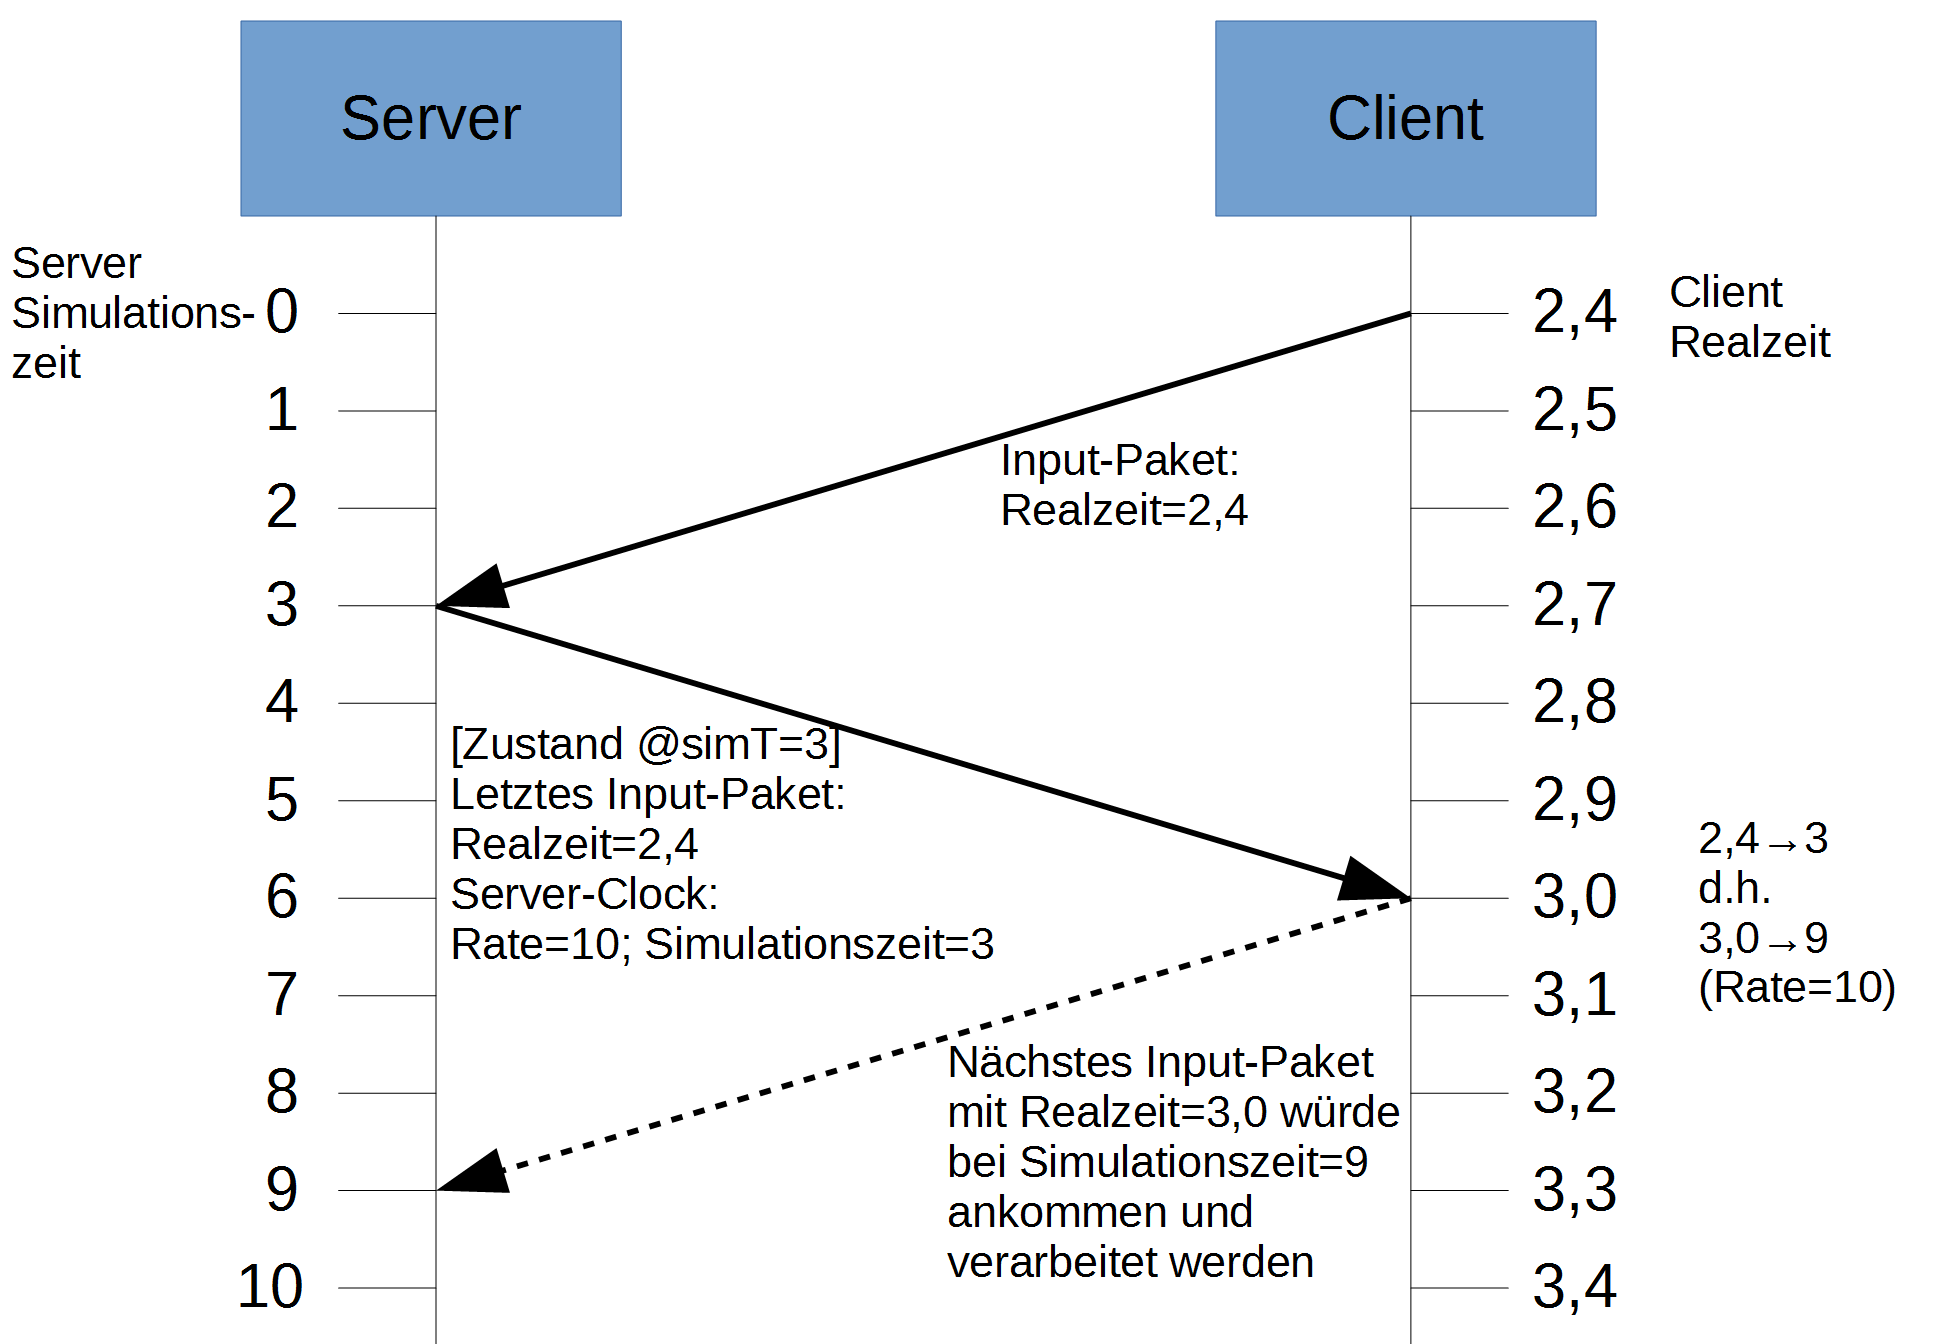
\includegraphics[width=0.75\textwidth]{./Zeichnung3a.png}
    \caption{Diagramm über Beispielsituation bei Simulationszeit-Uhrensynchronisation, mit Zeitversetzten Uhren wie in Abb. ~\ref{fig:zeichnung2a}. Gleiche Höhe entspricht Gleichzeitigkeit der echten Zeit. Dargestellt ist außerdem, wie der Client aus den Daten in den Synchronisierungspaketen diejenige Simulationszeit abschätzt, die dem Eintreffen (am Server) und Verarbeiten eines hypothetischen Pakets entspricht, wenn es sofort abgesendet werden würde.}
    \label{fig:zeichnung3a}
\end{figure}




Die graphische Ausgabe ist so gestaltet, dass anzuzeigende Informationsinhalte zur Anzeige zu einem bestimmten Simulationszeitpunkt inter- oder extrapoliert werden.
Es wird sich erhofft durch dieses Feature die Illusion von Gleichzeitigkeit zu erzeugen, in dem die graphische Ausgabe des Clients entsprechend der Durchschnittslatenz zum Server in der Zukunft gerendert wird. Auf dem Client durchgeführte Aktionen eines Benutzers können dadurch beim Eintreffen auf dem Server als gegenwärtig interpretiert werden.\\
Natürlich besteht dabei der Nachteil, dass ein Client u.U.~durch seine Vorhersage momentan falsche Szenen anzeigt. Das wird an dieser Stelle als der benötigte Trade-Off angesehen, um das atomare Problem der Latenz zu lösen.

Um die Zeit auf dem Client einzustellen, wird die in der Simulation enthaltene Uhr, welche die Simulationszeit steuert, synchronisiert.

%TODO sync protocol of clocks here


\subsection{Übertragung der Simulationsinhalte zum Client}
\label{sec:syncable}
Um die Simulationsinhalte übertragen zu können, wurde zunächst ein Interface entworfen, über das die Daten gelesen und geschrieben werden können. Das Interface wird hier Syncable genannt.
Zunächst müssen die möglichen Datensätze in Kategorien unterteilt werden:
\begin{itemize}
\item Update-Daten: Daten, die ein bestehendes Objekt in den neuen, aktuellen Zustand überführen (z.B. Position)
\item Vollständiger Datensatz: Daten, die übertragen werden müssen, um ein neues Objekt zu erstellen. Diese Daten beinhalten meist alle Update-Daten und beinhalten zusätzlich noch die Daten, die einmalig zur Initialisierung notwendig sind (z.B. Größe eines konkreten Gegners).
\end{itemize}
Bei einem Syncable gibt es also eine Serialisierungs- und Deserialisierungsmethode. Um die gewünschte Kategorie auszuwählen, wird beim Aufruf zur Serialisierung ein Parameter übergeben, der dieser Auswahl entspricht. Die jeweilige konkrete Implementierung sammelt die jeweils relevanten Daten und hängt sie an das übergebene Paket an. Für das Paket wird die Programmbibliothek SFML, genauer deren Netzwerkkomponente, verwendet. Dadurch werden auch plattformspezifische Details wie z.B. Endianness automatisch berücksichtigt. Bei der Deserialisierung passiert der umgekehrte Prozess: Die Daten werden aus dem Paket entnommen und jedes Objekt führt das Update entsprechend durch. Bei der vollständigen Deserialisierung gibt es jedoch eine Besonderheit: Das Objekt existiert vor dem Aufruf noch nicht, weshalb statt einer Methode ein spezieller Konstruktor vom jeweils konkreten Objekt zur Verfügung gestellt wird, der aus den Daten des Pakets das Objekt initialisiert.
Dies weist auf ein weiteres Problem hin: Es muss zur Erstellung der konkrete Konstruktor aufgerufen werden, nicht nur eine abstrakte Methode. Dafür wird eine Factory verwendet. Damit der Typ eines Objekts übertragen werden kann, muss dieser anhand einer ID mit einer abstrakten Methode abgefragt werden können. Die Factory auf der Gegenseite kann dann den konkreten Konstruktor für das Objekt aufrufen.
